%   Filename    : chapter_4.tex 

\chapter{Results and Discussions}
This chapter presents the results from the machine learning and deep learning analyses conducted on the preprocessed dataset. It includes an evaluation of various machine learning classifiers and the application of deep learning models for image-based classification. The primary focus is on identifying key predictors and assessing classification performance for sex identification in \textit{T. granosa}.

\section{Machine Learning Analysis}

This chapter outlines the results of preprocessing, training of machine learning models, and feature importance analysis, all conducted in Google Colab using Python. The dataset was preprocessed in Colab, and the training and evaluation of various classifiers were performed entirely within this environment.  This part of the paper includes five subsections: data exploration, statistical analysis, feature importance analysis, performance evaluation, and confusion matrix analysis.

\subsection{Data Exploration}

Exploratory data analysis was performed to characterize the dataset using visualizations to understand the patterns and correlations within the data. A correlation heatmap was created to assess the relationship between the predictors and the target variable.

The heatmap (see Figure~\ref{fig:heatmap}) revealed three features most correlated with the sex of \textit{T. granosa}: the width-height ratio (r = 0.18), the umbos-length ratio (r = 0.12), and the distance between the umbos (r = 0.12). Each of these features demonstrated a weak positive relationship with the target variable. 

\begin{figure}[!htbp]
	\centering
	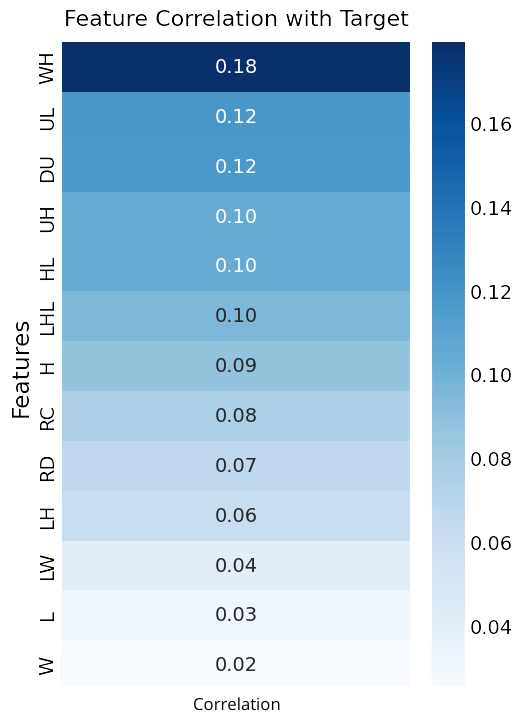
\includegraphics[width=0.4\textwidth]{figures/heatmap.png}
	\caption{Heatmap of morphometric correlations with \textit{T. granosa} sex.}
	\label{fig:heatmap}
\end{figure}

\subsection{Statistical Analysis}

As part of the exploratory data analysis, statistical testing confirmed that the dataset did not follow a normal distribution (\textit{see Table~\ref{tab:mann-whitney}}). Consequently, the Mann-Whitney U test was applied with a significance level of $\alpha = 0.05$ to compare male and female samples. Out of thirteen features, five showed statistically significant differences. These included: distance between umbos ($p = 0.025$), length-width ratio ($p = 0.011$), umbos-length ratio ($p = 0.019$), width-height ratio ($p = 0.003$), and umbos-height ratio ($p = 0.036$). 

It is important to note that statistical significance does not imply predictive importance. Therefore, further analysis, such as feature importance evaluation, was performed to identify the most informative predictors for classification.

\begin{table}[H]
	\centering
	\small % or \footnotesize or \scriptsize
	\begin{tabular}{lc}
		\hline
		\textbf{Variable} & \textbf{p-value} \\ \hline
		WH\_ratio & 0.003 \\
		LW\_ratio & 0.011 \\
		UL\_ratio & 0.019 \\
		Distance Umbos & 0.025 \\
		UH\_ratio & 0.036 \\
		HL\_ratio & 0.079 \\
		Length (Hinge Line) & 0.120 \\
		Height & 0.124 \\
		Rib Density & 0.181 \\
		Rib count & 0.251 \\
		Length & 0.334 \\
		LH\_ratio & 0.490 \\
		Width & 0.753 \\ \hline
		
	\end{tabular}
	
	\caption{Mann-Whitney U Test Results for Sex-Based Feature Comparison}
	\label{tab:mann-whitney}
\end{table}

\subsection{Feature Importance Analysis}

Feature importance was assessed using the Kruskal-Wallis test, a non-parametric method that is suitable for evaluating differences in distributions across groups when the data does not follow a normal distribution. This approach was chosen because of the non-normality of the dataset and its robustness in handling continuous and ordinal data without assuming homogeneity of variances. \cite{ribeiro2024}

The analysis showed that the width-to-height ratio (WH ratio) had the highest importance score, indicating it is the most statistically significant feature for distinguishing the sex of \textit{T. granosa}. Other notable features included the length-to-width ratio (LW ratio), umbo distance-to-length ratio (UL ratio), distance between the umbos, and umbo distance-to-height ratio (UH ratio), all of which contributed significantly to the classification task (refer to Figure~\ref{fig:kw}).

\begin{figure}[!htbp]
	\centering
	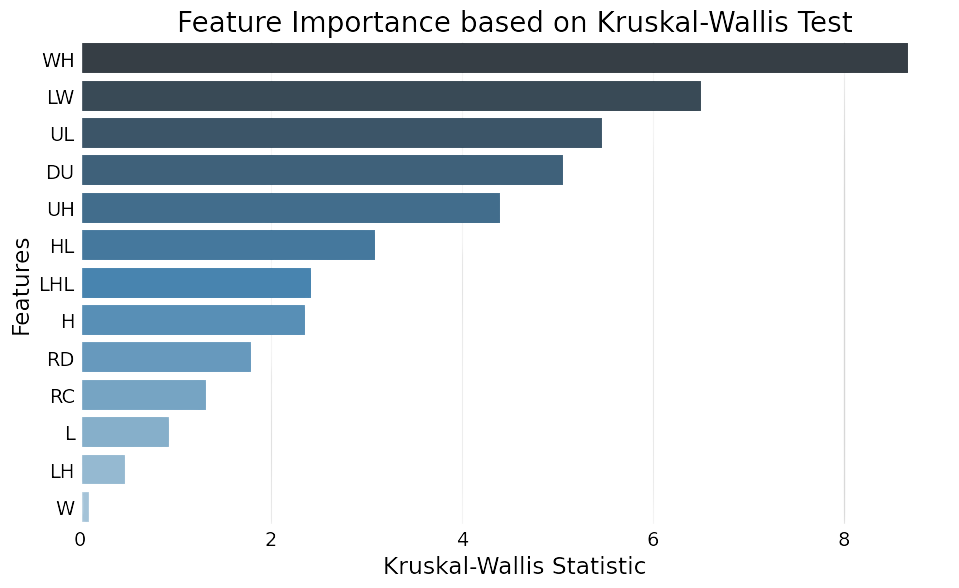
\includegraphics[width=1.0\textwidth]{figures/kw.png}
	\caption{Feature importance scores using the Kruskal-Wallis test.}
	\label{fig:kw}
\end{figure}

\subsection{Performance Evaluation}
\label{tab:performance-eval}

\begin{table}[H]
	\centering
	\resizebox{\textwidth}{!}{
		\begin{tabular}{lcccccc}
			\hline
			\textbf{Model} & \textbf{Accuracy (\%)} & \textbf{Precision (\%)} & \textbf{Recall (\%)} & \textbf{F1-Score (\%)} \\ \hline
			Support Vector Machine   & 58.62 & 58.62 & 58.62 & 58.44 \\
			Logistic Regression      & 57.83 & 57.83 & 57.83 & 57.61 \\
			K-Nearest Neighbors      & 51.18 & 51.31 & 51.18 & 50.77 \\
			Extra Trees              & 59.07 & 59.54 & 59.07 & 58.45 \\
			Random Forest            & 59.85 & 59.99 & 59.85 & 59.80 \\
			\cellcolor{celadon}Gradient Boosting        & \cellcolor{celadon}61.03 & \cellcolor{celadon}61.32 & \cellcolor{celadon}61.03 & \cellcolor{celadon}60.81 \\
			AdaBoost & 60.63 & 60.98 & 60.63 & 60.39 \\
			\hline
		\end{tabular}
	}
	\caption{Performance Metrics for Models with All 13 Features}
	\label{tab:performance-13-features}
\end{table}

Table~\ref{tab:performance-13-features} shows the performance metrics of different machine learning models trained using all 13 features from the dataset. Among the models, Gradient Boosting achieved the highest accuracy of 61.03\%, along with strong precision, recall, and F1-score values. AdaBoost also performed competitively, with an accuracy of 60.63\%. These results highlight the effectiveness of ensemble methods such as Gradient Boosting and AdaBoost when utilizing the full feature set, likely because of their capability to combine multiple weak learners into a more robust predictive model \cite{hussain2024}.  

\begin{table}[H]
	\centering
	\resizebox{\textwidth}{!}{
		\begin{tabular}{lcccccc}
			\hline
			\textbf{Model} & \textbf{Accuracy (\%)} & \textbf{Precision (\%)} & \textbf{Recall (\%)} & \textbf{F1-Score (\%)} \\ \hline
			Support Vector Machine   & 63.77 & 64.47 & 63.77 & 63.42 \\
			Logistic Regression      & 63.75 & 63.87 & 63.75 & 63.70 \\
			\cellcolor{celadon}K-Nearest Neighbors      & \cellcolor{celadon}64.16 & \cellcolor{celadon}64.97 & \cellcolor{celadon}64.16 & \cellcolor{celadon}63.75 \\
			Extra Trees              & 61.04 & 61.68 & 61.04 & 60.67 \\
			Random Forest            & 61.01 & 61.12 & 61.01 & 60.91 \\
			Gradient Boosting        & 64.15 & 64.24 & 64.15 & 64.01 \\
			AdaBoost                 & 61.02 & 61.26 & 61.02 & 60.82 \\
			\hline
		\end{tabular}
	}
	\caption{Performance Metrics for Models with 5 Features}
	\label{tab:performance-5-features}
\end{table}

Table~\ref{tab:performance-5-features} presents the performance of the same models using only the top five features identified through Kruskal-Wallis feature importance analysis. The selected features are the distance between the umbos, length-to-width ratio, width-to-height ratio, umbo distance-to-height ratio, and umbo distance-to-length ratio.

Interestingly, the overall performance of the models improved when using only the top 5 features compared to using all 13. K-Nearest Neighbors (KNN) achieved the best results with an accuracy of 64.16\%, precision of 64.97\%, recall of 64.16\%, and an F1-score of 63.75\%. Gradient Boosting followed closely behind. These findings suggest that reducing the feature set to the most relevant variables helped simplify the models, improved generalization, and enhanced predictive performance—particularly for KNN, which showed a notable improvement over its earlier results with the full feature set.

\subsection{Confusion Matrix Analysis}

\begin{figure}[!htbp]
	\centering
	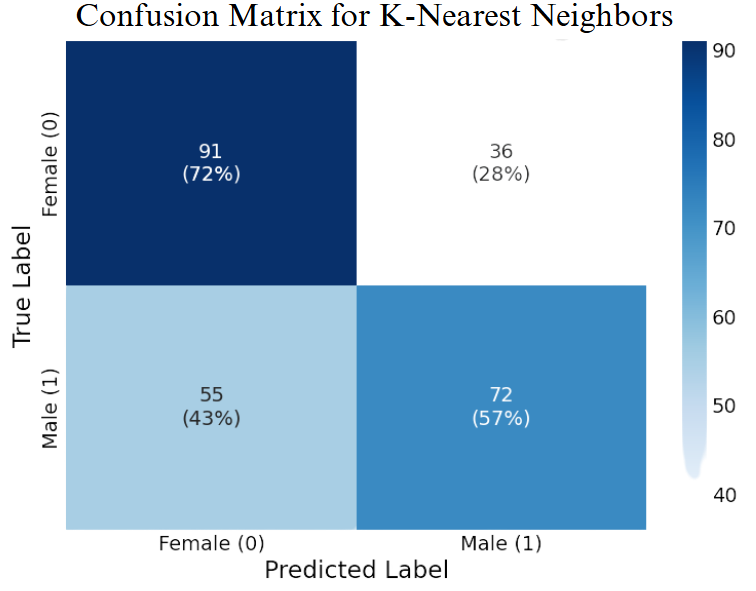
\includegraphics[width=0.8\textwidth]{figures/confusion_matrix_ml.png}
	\caption{KNN confusion matrix for \textit{T. granosa} sex classification.}
	\label{fig:cm_ml}
\end{figure}

Figure~\ref{fig:cm_ml} summarizes the performance of the K-Nearest Neighbors model in classifying \Tgranosa based on their sex, where 0 represents female samples and 1 represents male samples. From the matrix, we observe that out of all the actual female samples (true label 0), 91 were correctly predicted as female (true positive for class 0), while 36 were incorrectly classified as male (false negative for class 0). On the other hand, out of all the actual male samples (true label 1), 72 were correctly predicted as male (true positive for class 1), while 55 were incorrectly classified as female (false negative for class 1).

\section{Deep Learning Analysis}
This section presents the performance of the Convolutional Neural Network (CNN) model in classifying the sex of \Tgranosa based on shell morphology. The analysis evaluates the model's ability to distinguish between male and female shell images using various evaluation metrics. This part of the paper includes six subsections: baseline model, comparison of individual and combined angles, training result and hyperparameter tuning, proposed model, learning rates and training behavior per fold, and visualizations.

The machine learning analysis (see Figure~\ref{tab:performance-5-features}) revealed that five of the original features produced significant results. The K-Nearest Neighbor (KNN) model achieved an accuracy of 64.16\%, precision of 64.97\%, recall of 64.16\%, and an F1 score of 63.75\%. This section compares the model's performance across different angles based on the results of the machine learning and feature importance analysis.

\subsection{Baseline Model}
This section presents the baseline model with a batch size of 16 and 20 epochs, which will serve as the starting point for comparison and provide a guideline for hyperparameter tuning. The focus will be on one of the angles, specifically the Left Lateral view, since the feature importance analysis using the Kruskal-Wallis Test indicated that the width-to-height ratio had the highest importance score, which is most visible from the Left Lateral view.

\begin{table}[H]
	\centering
	\resizebox{\textwidth}{!}{
		\begin{tabular}{lcccccc}
			\hline
			\textbf{Dataset} & \textbf{Accuracy (\%)} & \textbf{Precision (\%)} & \textbf{Recall (\%)} & \textbf{F1-Score (\%)}  & \textbf{AUC score (\%)}  & \textbf{Loss (\%)} \\ \hline
			Unbalanced   & 65.27 & 71.82 & 58.99 & 63.99 & 73.08 & 0.6122 \\
			\rowcolor{celadon}Balanced     & 67.34 & 69.43 & 64.06 & 65.60 & 74.31 & 0.5981 \\
			\hline
		\end{tabular}
	}
	\caption{Performance Metrics for Unbalanced vs. Balanced Datasets (Batch Size: 16, Epochs: 20)}
	\label{tab:unbalanced-balanced}
\end{table}

The unbalanced dataset, which consisted of 144 male samples and 127 female samples, achieved an accuracy of 65.27\%, precision of 71.82\%, recall of 58.99\%, an F1-score of 63.99\%, an AUC score of 73.08\%, and a loss of 0.6122. However, to address the class imbalance and enhance model performance, random undersampling was performed. This approach resulted in improved performance metrics for the balanced dataset, with an accuracy of 67.34\%, precision of 69.43\%, a recall of 64.06\%, an F1-score of 65.60\%, an AUC score of 74.31\%, and a lower loss of 0.5981.

\subsection{Comparison of Individual and Combined Angles}
Using the same batch size and number of epochs, performance was compared across all individual angles and the combination of the two highest-performing angles based on accuracy, using a balanced dataset. For the combined analysis, samples from the two selected angles were placed side by side, and a new dataset folder was created for male and female samples. 

\begin{table}[H]
	\centering
	\resizebox{\textwidth}{!}{
		\begin{tabular}{lcccccc}
			\hline
			\textbf{Angle} & \textbf{Accuracy (\%)} & \textbf{Precision (\%)} & \textbf{Recall (\%)} & \textbf{F1-Score (\%)} & \textbf{AUC score (\%)} & \textbf{Loss (\%)} \\ \hline
			Dorsal 	 				& 66.54 & 63.76 & \cellcolor{celadon}77.88 & \cellcolor{celadon}69.96 & 73.09 & 0.6152 \\
			Ventral  				& 67.30 & 69.33 & 66.18 & 66.53 & \cellcolor{celadon}74.87 & 0.6159 \\
			Anterior  				& 51.57 & 31.11 & 6.31  & 10.02 & 65.87 & 0.6825 \\
			Posterior  				& 61.43 & 63.48 & 51.17 & 54.25 & 70.12 & 0.6257 \\
			Left Lateral  			& \cellcolor{celadon}67.34 & \cellcolor{celadon}69.43 & 64.06 & 65.60 & 74.31 & 0.5981 \\
			Right Lateral  			& 65.37 & 67.18 & 59.82 & 62.99 & 71.02 & 0.6115 \\
			Ventral + Left Lateral  & 62.60 & 67.02 & 57.85 & 58.57 & 70.37 & 0.6433 \\
			\hline
		\end{tabular}
	}
	\caption{Performance Metrics for Individual and Combined Angles (Batch Size: 16, Epochs: 20)}
	\label{tab:individual-combined}
\end{table}

Table~\ref{tab:individual-combined} presents the performance metrics for each individual angle and the combination of the two highest-performing angles in terms of accuracy. The Left Lateral view achieved the highest accuracy (67.34\%) and precision (69.43\%), while the Dorsal view obtained the highest recall (77.88\%) and F1-score (69.96\%). Meanwhile, the Ventral view recorded the highest AUC score (74.87\%), indicating its strong ability to distinguish between classes.
Combining the Ventral and Left Lateral views resulted in an overall accuracy of 62.60\%, suggesting that while combined images may provide complementary information, individual angle views still outperformed the combined views under the current experimental setup.

\subsection{Training Result and Hyperparameter Tuning}
The Left Lateral angle was selected for further optimization. Several experiments were conducted by tuning hyperparameters such as batch size, number of epochs, and activation functions. Each adjustment was compared against the baseline model to enhance performance and develop a robust CNN for sex classification of \textit{T. granosa}.

The Left Lateral angle was chosen because it achieved the highest accuracy and precision among all individual views, and because the Kruskal-Wallis feature importance analysis indicated that the width-to-height ratio, a feature most visible from the lateral perspective, was the most significant morphological trait for classification. Therefore, focusing on this view was expected to maximize the model's learning capacity and improve classification performance.

\noindent\textbf{A. Batch Size and Number of Epochs}

\begin{table}[H]
	\centering
	\resizebox{\textwidth}{!}{
		\begin{tabular}{lccccccc}
			\hline
			\textbf{Batch Size} & \textbf{No. of Epoch} & \textbf{Accuracy (\%)} & \textbf{Precision (\%)} & \textbf{Recall (\%)} & \textbf{F1-Score (\%)} & \textbf{AUC score (\%)} & \textbf{Loss (\%)} \\ \hline
			16 & 20 & 67.34 & 69.43 & 64.06 & 65.60 & 74.31 & 0.5981 \\
			16 & 30 & 67.73 & 70.17 & 64.06 & 65.72 & 75.76 & 0.5900 \\
			16 & 50 & 67.73 & 70.17 & 64.06 & 65.72 & 75.76 & 0.5900  \\
			32 & 20 & 68.13 & 72.25 & 58.95 & 62.34 & 74.76 & 0.6041 \\
			32 & 30 & 71.28 & 73.17 & 66.89 & 68.27 & 76.76 & 0.5832 \\
			\cellcolor{celadon}32 & \cellcolor{celadon}50 & \cellcolor{celadon}71.68 & \cellcolor{celadon}72.52 & \cellcolor{celadon}69.29 & \cellcolor{celadon}69.12 & \cellcolor{celadon}77.34 & \cellcolor{celadon}0.5824 \\
			64 & 20 & 56.71 & 65.96 & 36.83 & 41.46 & 71.28 & 0.6692 \\
			64 & 30 & 57.95 & 61.94 & 48.12 & 52.66 & 71.22 & 0.6241 \\
			64 & 50 & 61.10 & 62.68 & 56.12 & 56.83 & 73.46 & 0.6086 \\
			\hline
		\end{tabular}
	}
	\caption{Effect of Batch Size and Epoch Values on CNN Model Performance}
	\label{tab:batchsize-epoch}
\end{table}

Table~\ref{tab:batchsize-epoch} shows the results indicating that a batch size of 32 with 50 epochs achieved the best overall performance, with an accuracy of 71.68\%, a precision of 72.52\%, a recall of 69.29\%, an F1-score of 69.12\%, and AUC score of 77.34\%.

In contrast, increasing the batch size to 64 resulted in lower recall and F1-scores, suggesting that smaller batch Sizes (16 or 32) are more effective for this dataset. A moderate batch size of 32 allowed the model to generalize better and maintain stable learning, while too large batch sizes may have led to underfitting.

\noindent\textbf{B. Activation Functions}

\begin{table}[H]
	\centering
	\resizebox{\textwidth}{!}{
		\begin{tabular}{lcccccc}
			\hline
			\textbf{Activation Functions} & \textbf{Accuracy (\%)} & \textbf{Precision (\%)} & \textbf{Recall (\%)} & \textbf{F1-Score (\%)}  & \textbf{AUC score (\%)}  & \textbf{Loss (\%)} \\ \hline
			\rowcolor{celadon}ReLU  & 71.68 & 72.52 & 69.29 & 69.12  & 77.34 & 0.5824 \\
			ELU   					& 53.14 & 32.91 & 53.08 & 39.95  & 58.23 & 0.6796 \\
			PreLU   				& 62.64 & 66.59 & 50.43 & 56.96  & 72.33 & 0.6162 \\
			\hline
		\end{tabular}
	}
	\caption{Performance Metrics for Different Activation Functions (Batch Size: 32, Epochs: 50)}
	\label{tab:activation-function}
\end{table}

Table~\ref{tab:activation-function} the performance of different activation functions applied to the CNN model trained with a batch size of 32 and 50 epochs. Based on the results, the ReLU activation function achieved the best overall performance, with an accuracy of 71.68\%, precision of 72.52\%, recall of 69.29\%, F1-score of 69.12\%, and AUC score of 77.34\%, along with the lowest loss at 0.5824. This suggests that ReLU remains an effective activation function for the classification of \textit{T. granosa}, outperforming both ELU and PReLU in this setup.

\subsection{Proposed Model}
This section presents the performance evaluation of the proposed Convolutional Neural Network (CNN) model, trained with a batch size of 32, 50 epochs, and using the ReLU activation function. The model’s effectiveness was assessed through 5-fold cross-validation to ensure robustness and generalizability across different data partitions. 

\begin{table}[H]
	\centering
	\resizebox{\textwidth}{!}{
		\begin{tabular}{lcccccc}
			\hline
			\textbf{Fold no.} & \textbf{Accuracy (\%)} & \textbf{Precision (\%)} & \textbf{Recall (\%)} & \textbf{F1-Score (\%)}  & \textbf{AUC score (\%)}  & \textbf{Loss (\%)} \\ \hline
			Fold 1  & 76.47 & 70.59 & 92.31 & 80.00  & 73.08 & 0.5975 \\
			Fold 2  & 62.75 & 70.59 & 46.15 & 55.81  & 71.85 & 0.6202 \\
			Fold 3  & 78.43 & 75.00 & 84.00 & 79.25  & 84.92 & 0.5392 \\
			Fold 4  & 62.75 & 71.43 & 40.00 & 51.28  & 71.08 & 0.6331 \\
			Fold 5  & 78.00 & 75.00 & 84.00 & 79.25  & 85.76 & 0.5219 \\
			\hline
		\end{tabular}
	}
	\caption{Per-Fold Performance Metrics (Batch Size: 32, Epochs: 50, Activation Function: ReLU)}
	\label{tab:per-fold}
\end{table}

The proposed model consistently achieved high performance in Folds 1, 3, and 5, with accuracies above 76\% and strong recall and AUC scores, demonstrating its potential for reliable sex identification of \textit{T. granosa}. The slight variation in performance across folds may be attributed to differences in data distribution, emphasizing the importance of further data augmentation and balancing for future work.

\subsection{Learning Rates and Training Behavior per Fold}
This section presents the learning rate adjustments, early stopping events, and best epoch selections for each fold during the 5-fold cross-validation of the proposed model. During training, the ReduceLROnPlateau callback was employed to monitor the validation loss and automatically reduce the learning rate when performance plateaued. Additionally, EarlyStopping was utilized to halt training once no further improvement was observed after a set patience, and the model weights were restored from the end of the best-performing epoch to ensure optimal performance.

The following table summarizes the epochs where learning rate reductions occurred, the adjusted learning rates, the epochs at which early stopping took place, and the best epochs from which model weights were restored for each fold.

\begin{table}[H]
	\centering
	\resizebox{\textwidth}{!}{
		\begin{tabular}{lcccc}
			\hline
			\textbf{Fold no.} & \begin{tabular}[c]{@{}c@{}}\textbf{Epoch}\\\textbf{(LR Reduced)}\end{tabular} & \begin{tabular}[c]{@{}c@{}}\textbf{Learning Rate}\\\textbf{After Reduction}\end{tabular} & \begin{tabular}[c]{@{}c@{}}\textbf{Early}\\\textbf{Stopping Epoch}\end{tabular} & \begin{tabular}[c]{@{}c@{}}\textbf{Best Epoch}\\\textbf{(Restored)}\end{tabular} \\ \hline
			Fold 1 & \begin{tabular}[c]{@{}c@{}}20\\23\end{tabular} & \begin{tabular}[c]{@{}c@{}}0.0005000\\0.0002500\end{tabular} & 25 & 17 \\ \hline
			Fold 2 & \begin{tabular}[c]{@{}c@{}}9\\14\\17\end{tabular} & \begin{tabular}[c]{@{}c@{}}0.0005000\\0.0002500\\0.0001250\end{tabular} & 19 & 11 \\ \hline
			Fold 3 & \begin{tabular}[c]{@{}c@{}}15\\18\end{tabular} & \begin{tabular}[c]{@{}c@{}}0.0005000\\0.0002500\end{tabular} & 20 & 12 \\ \hline
			Fold 4 & \begin{tabular}[c]{@{}c@{}}12\\15\\27\\30\end{tabular} & \begin{tabular}[c]{@{}c@{}}0.0005000\\0.0002500\\0.0001250\\0.0000625\end{tabular} & 32 & 24 \\ \hline
			Fold 5 & \begin{tabular}[c]{@{}c@{}}20\\23\end{tabular} & \begin{tabular}[c]{@{}c@{}}0.0005000\\0.0002500\end{tabular} & 25 & 17 \\ \hline
		\end{tabular}
	}
	\caption{Learning Rate Reductions, Early Stopping, and Best Epochs per Fold During 5-Fold Cross-Validation}
	\label{tab:learning-folds}
\end{table}


\subsection{Visualizations}

\begin{figure}[!htbp]
	\centering
	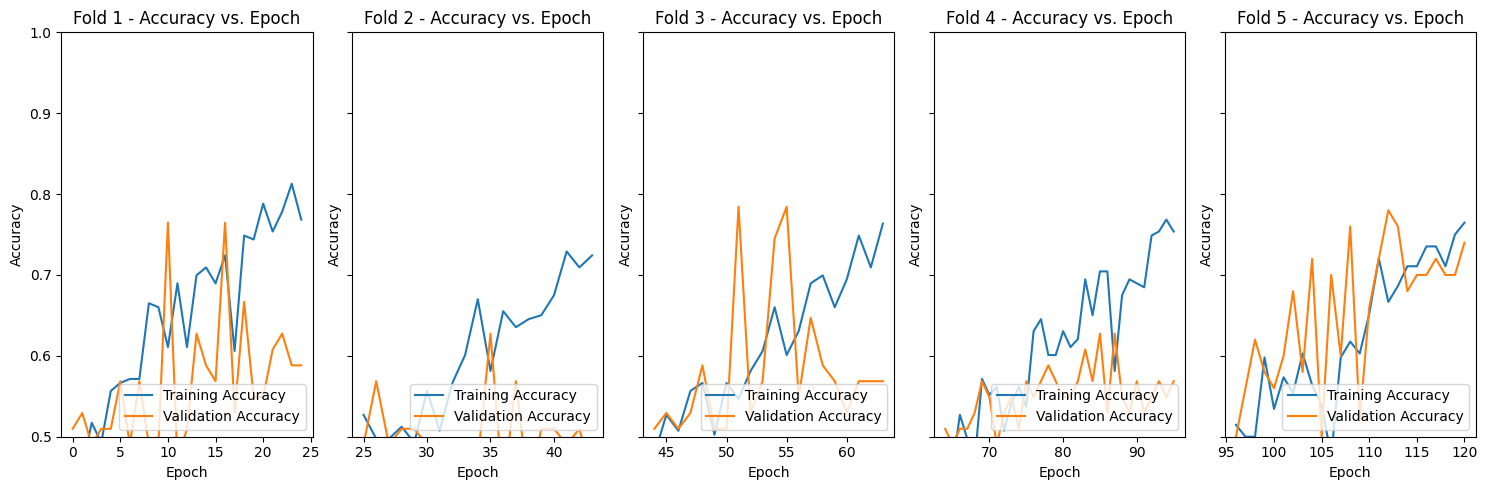
\includegraphics[width=0.8\textwidth]{figures/acc_epoch.png}
	\caption{Training and validation accuracy per fold.}
	\label{fig:tvapf}
\end{figure}

Figure~\ref{fig:tvapf} shows the performance of the model in the training and validation in terms of accuracy across five folds. The graph across folds displays a consistent upward trend for the training accuracy. However, there is an observable change in the performance, particularly in Folds 1 and 2, where it shows a slight downward trend in the validation accuracy.

\begin{figure}[!htbp]
	\centering
	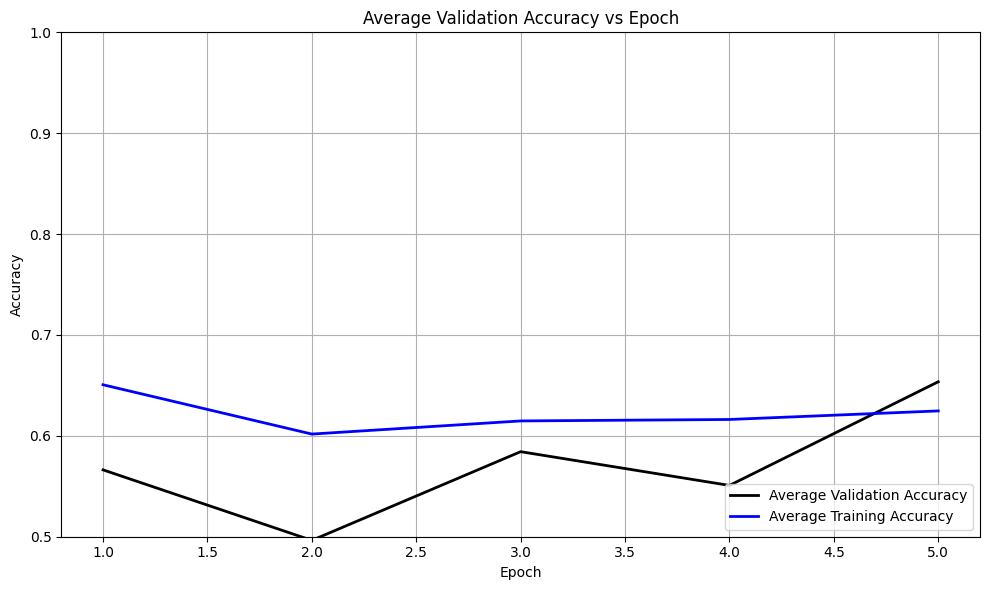
\includegraphics[width=0.8\textwidth]{figures/avg_acc.png}
	\caption{Average training and validation accuracy across folds.}
	\label{fig:atvaaf}
\end{figure}

Figure~\ref{fig:atvaaf} shows the average performance of the model in both training and accuracy in terms of accuracy across five folds. Similar to the individual performances, there is an observable upward trend, which shows that the accuracy score improves with the number of folds. The validation accuracy shows a downward and upward trend that shows that it gradually improves on later epochs. The accuracy in the training is slightly higher than the accuracy when validating the model, it indicates that the model learns during training.

\begin{figure}[!htbp]
	\centering
	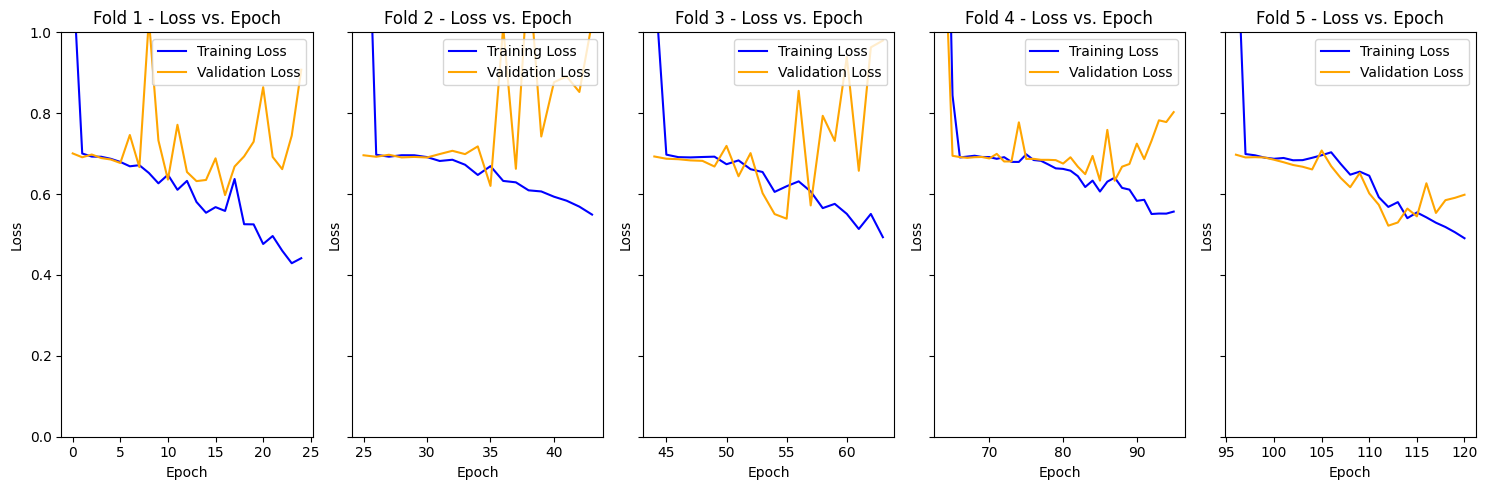
\includegraphics[width=0.8\textwidth]{figures/loss_epoch.png}
	\caption{Training and validation loss per fold.}
	\label{fig:tvlpf}
\end{figure}

Figure~\ref{fig:tvlpf} shows the performance of the model in the training and validation in terms of the training and validation loss across five folds. The graph across folds displays a consistent downward trend for the training loss. On the other hand, there is an observable change in the performance, especially in Folds 1,2,3, and 4, where it shows an upward trend in the validation loss. This is an implication for the learning performance of the model, as it may not be learning effectively. 

\begin{figure}[!htbp]
	\centering
	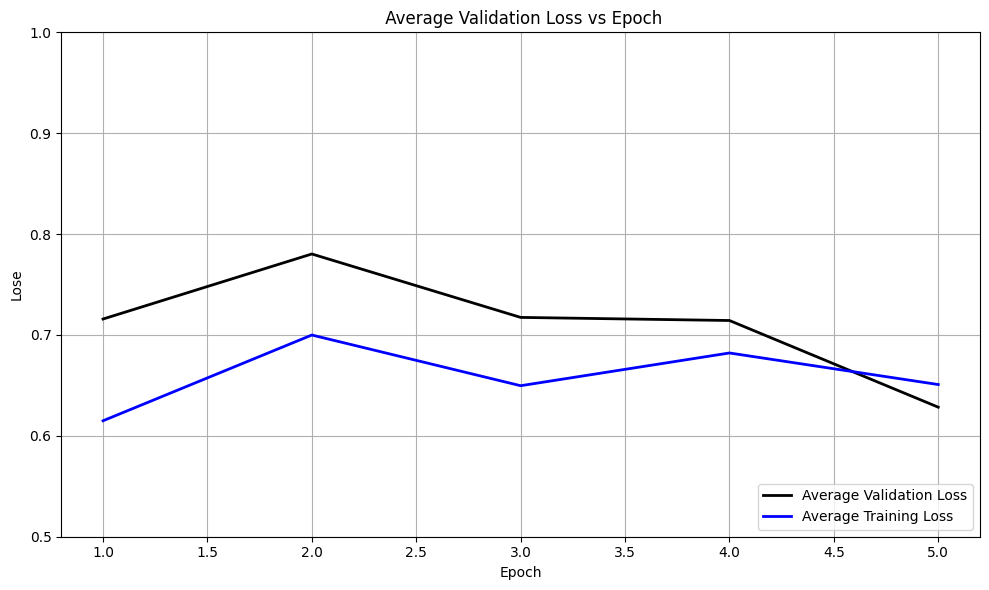
\includegraphics[width=0.8\textwidth]{figures/avg_loss.png}
	\caption{Average training and validation loss across folds.}
	\label{fig:atvlaf}
\end{figure}

Figure~\ref{fig:atvlaf} shows the average performance of the model in both the training and validation in terms of loss across five folds. There is an observable downward trend in both the average loss for training and validation. Additionally, the average training loss is slightly lower than the average validation loss.

\begin{figure}[!htbp]
	\centering
	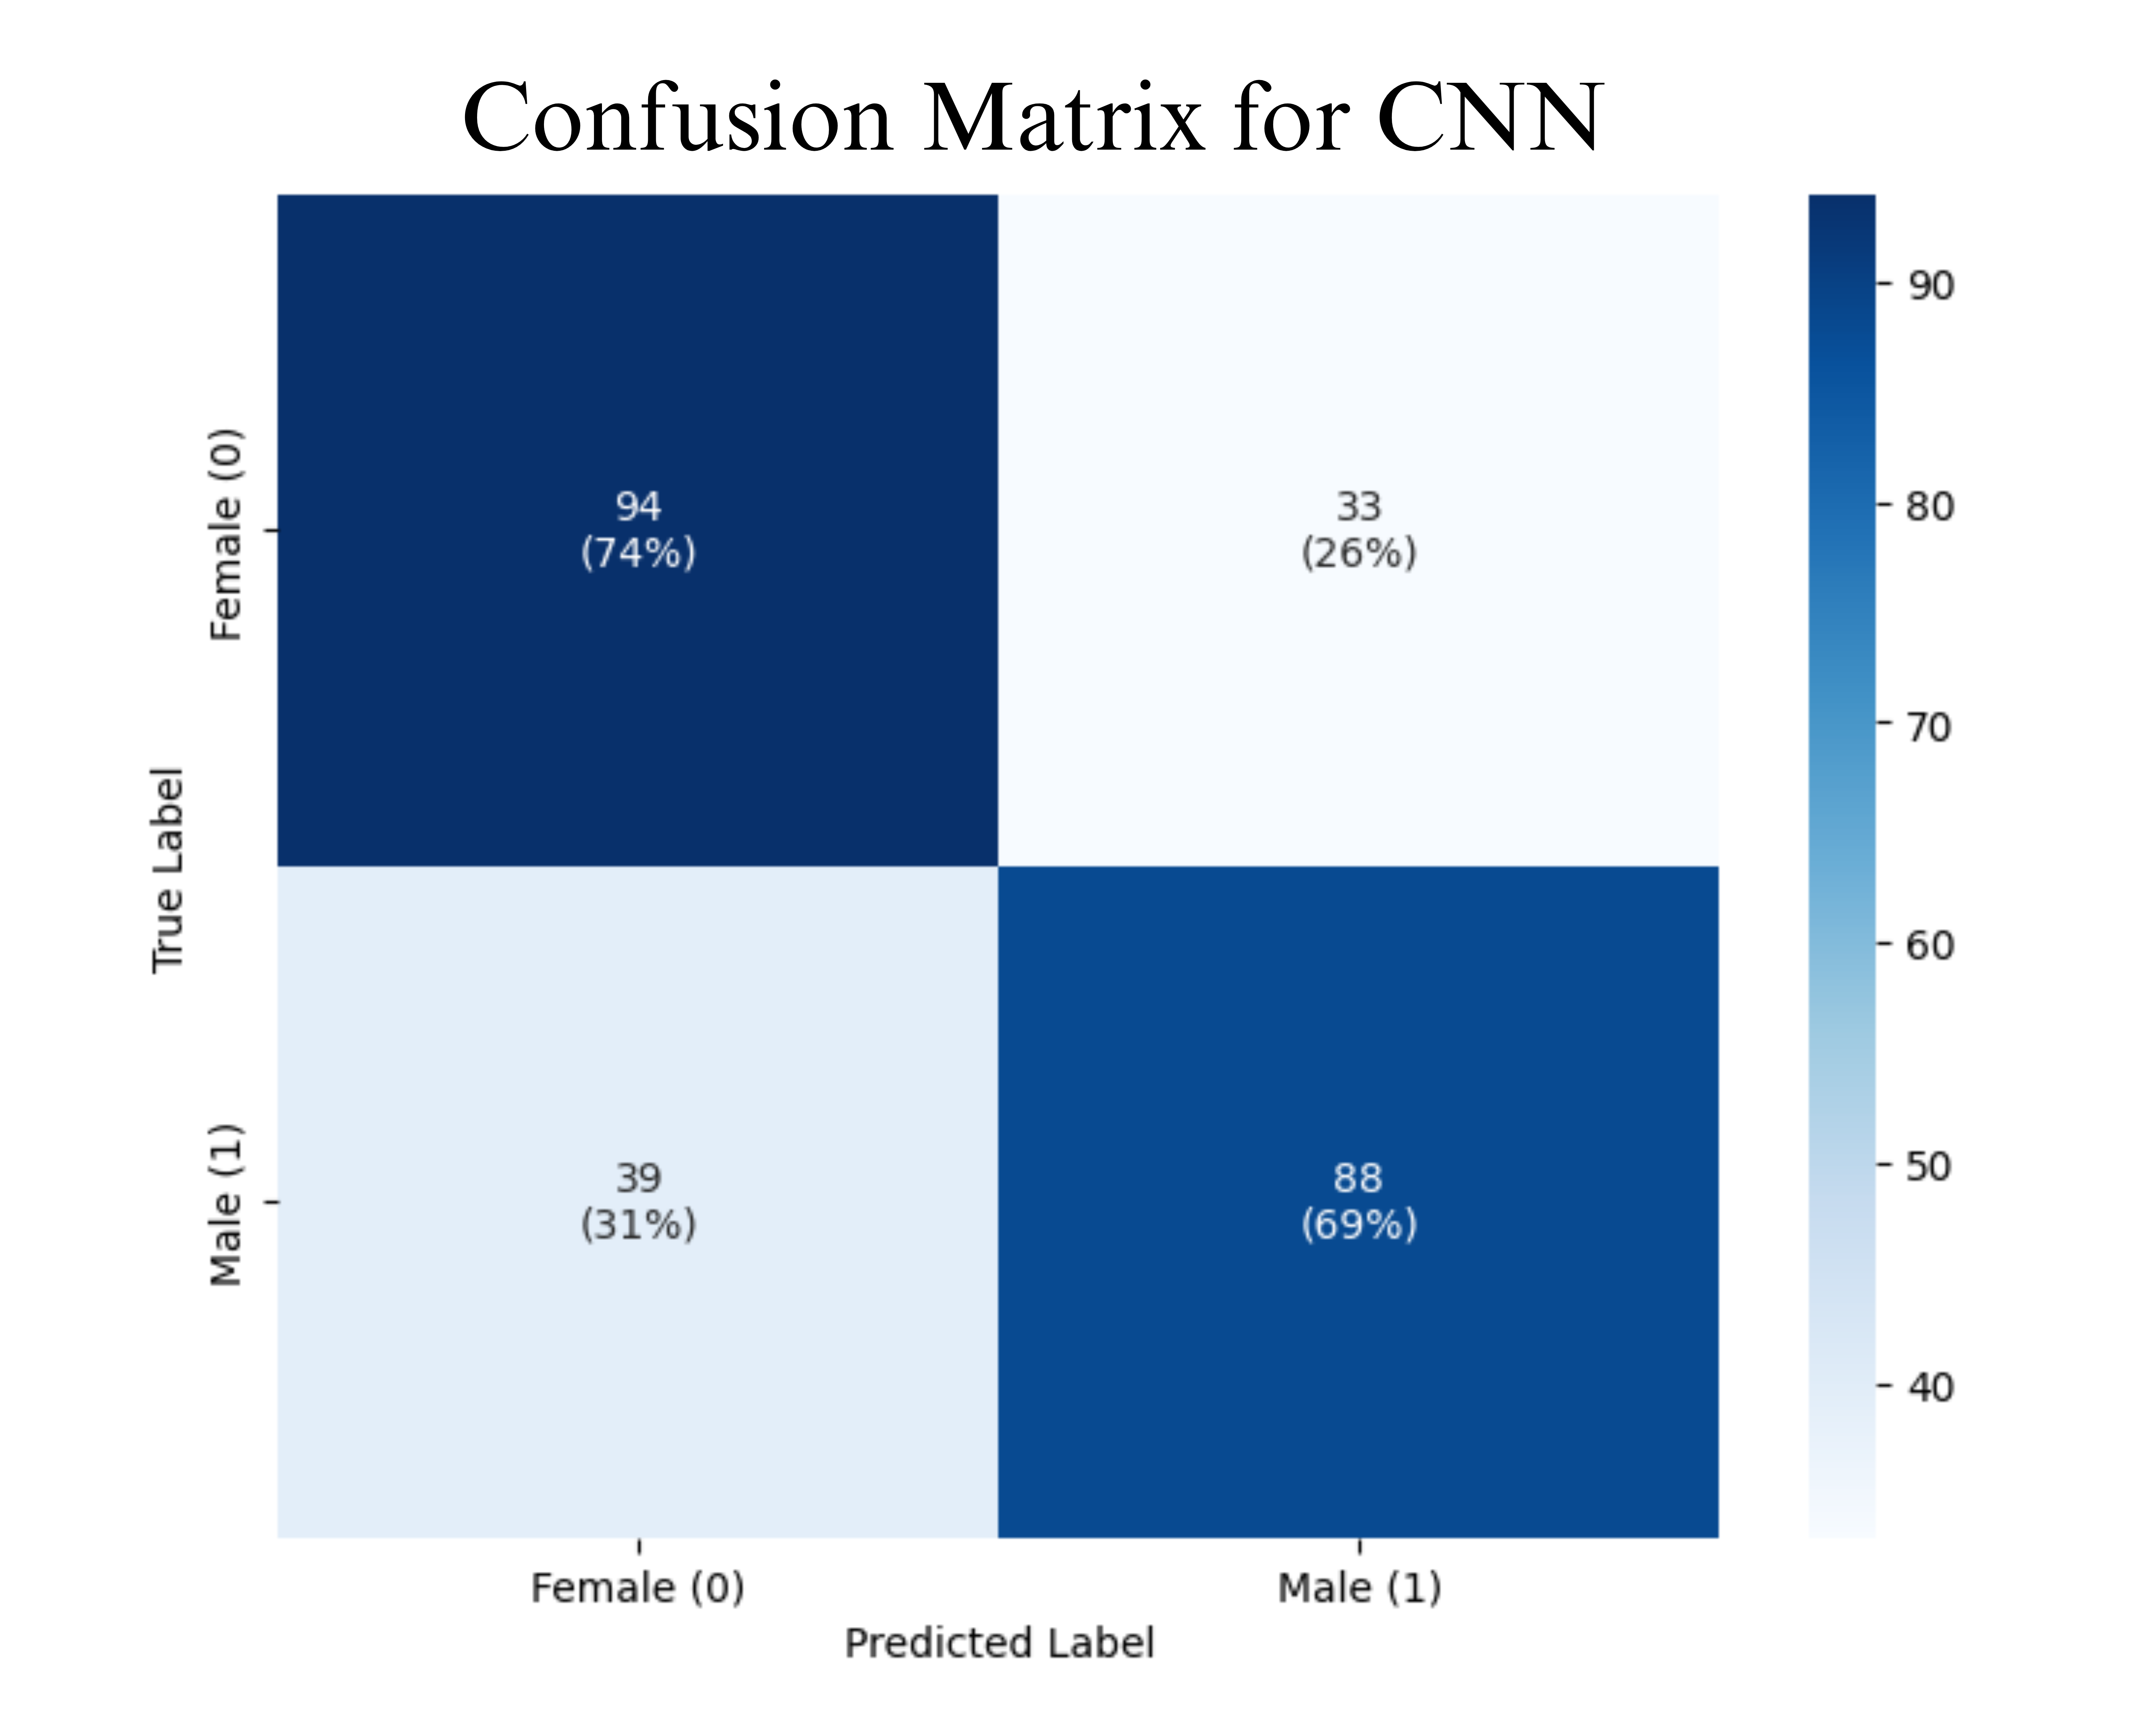
\includegraphics[width=0.8\textwidth]{figures/cm_dl.png}
	\caption{Confusion matrix for final model predictions.}
	\label{fig:cm_dl}
\end{figure}

Figure~\ref{fig:cm_dl} shows the confusion matrix for the true class label and predicted class label. The matrix shows the correctly predicted male and female samples along with their corresponding percentages. There is an observable trend where females have slightly higher true positives compared to males in the number and percentages for the correctly classified male and female samples, which are 94 and 88, corresponding to 74\% and 69\%, respectively. Additionally, the false classified samples were 33 for females and 39 for males, respectively accounting for 26\% and 31\%.

\begin{figure}[!htbp]
	\centering
	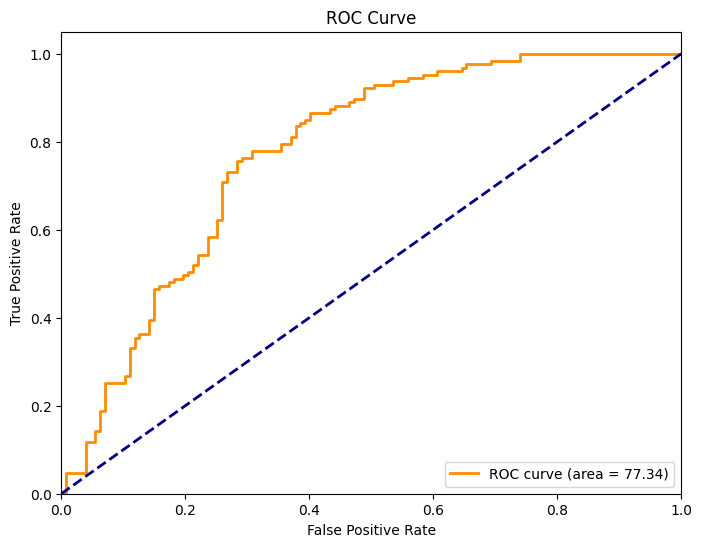
\includegraphics[width=0.8\textwidth]{figures/roc.png}
	\caption{ROC curve with AUC score for the proposed model.}
	\label{fig:roc_auc}
\end{figure}

Figure~\ref{fig:roc_auc} shows the ROC Curve shows the ability of the proposed model to correctly identify the true positives, which can help determine the tradeoff between specificity and sensitivity. It will also determine the validity of the model, that it is not predicting based only on random chances. The range of AUC ROC is between 0.5 and 1. The model was able to achieve a score of 0.7734, which is better than random chances and an indication that the model is performing reasonably. 

\section{Discussions}

This study aimed to develop a non-invasive method for identifying the sex of \textit{T. granosa} using machine learning, deep learning, and computer vision technologies. The dataset was manually curated by the researchers, including both the linear measurements and the images captured from six different angles.

The machine learning approach revealed that using five key features, selected through statistical tests (Mann-Whitney U-test and Kruskal-Wallis test), outperformed models trained on all 13 features. The K-nearest neighbors (KNN) classifier, using only these five features, achieved an accuracy of 64.16\%, precision of 64.97\%, recall of 64.16\%, and an F1-score of 63.57\%. These results indicate that a more focused set of features can enhance model performance, confirming the potential of non-invasive sex identification using linear measurements.

Further deep learning experiments explored how different image angles impacted performance. The study found that the Left Lateral view consistently produced the best results, with an accuracy of 71.68\%, precision of 72.52\%, recall of 69.29\%, F1-score of 69.12\%, and an AUC score of 77.34\%. This suggests that optimizing image angles is crucial, and combining multiple angles did not significantly improve the model’s performance. Data augmentation and regularization techniques, such as early stopping, helped improve the model's generalization and prevent overfitting.

The findings are significant because they demonstrate the feasibility of a non-invasive, accurate, and efficient sex identification method for \textit{T. granosa}. This approach aligns with sustainable aquaculture practices by reducing the need for harmful physical sex-identifying methods. By integrating machine learning with deep learning image analysis, this study provides a valuable model for non-invasive sex identification which could be applied to other species in aquaculture as well.

When compared to similar existing studies such as the gender classification method for Chinese mitten crab using deep learning CNN (Cui \textit{et al.}, 2020), there are notable differences in methodology. The crab study used grayscale images and a CNN with three convolutional layers, achieving 98.90\% accuracy. In contrast, this study utilized a hybrid approach combining machine learning with deep learning CNNs, trained on RGB images (256$\times$256), and a deeper CNN architecture. Despite achieving lower accuracy (71.68\%), this variation could be due to the subtler morphological differences between male and female \textit{T. granosa}, or possibly due to image quality limitations and sample size.

There are limitations in this study, particularly the size of the dataset (271 samples) and the reliance on six fixed image angles. These constraints may not fully represent the morphological variability across different populations or environments. Despite these limitations, the study successfully demonstrates that combining machine learning and deep learning with computer vision can provide a reliable and non-invasive solution for sex identification in \textit{T. granosa}.